\documentclass[twoside]{book}

% Packages required by doxygen
\usepackage{fixltx2e}
\usepackage{calc}
\usepackage{doxygen}
\usepackage[export]{adjustbox} % also loads graphicx
\usepackage{graphicx}
\usepackage[utf8]{inputenc}
\usepackage{makeidx}
\usepackage{multicol}
\usepackage{multirow}
\PassOptionsToPackage{warn}{textcomp}
\usepackage{textcomp}
\usepackage[nointegrals]{wasysym}
\usepackage[table]{xcolor}

% Font selection
\usepackage[T1]{fontenc}
\usepackage[scaled=.90]{helvet}
\usepackage{courier}
\usepackage{amssymb}
\usepackage{sectsty}
\renewcommand{\familydefault}{\sfdefault}
\allsectionsfont{%
  \fontseries{bc}\selectfont%
  \color{darkgray}%
}
\renewcommand{\DoxyLabelFont}{%
  \fontseries{bc}\selectfont%
  \color{darkgray}%
}
\newcommand{\+}{\discretionary{\mbox{\scriptsize$\hookleftarrow$}}{}{}}

% Page & text layout
\usepackage{geometry}
\geometry{%
  a4paper,%
  top=2.5cm,%
  bottom=2.5cm,%
  left=2.5cm,%
  right=2.5cm%
}
\tolerance=750
\hfuzz=15pt
\hbadness=750
\setlength{\emergencystretch}{15pt}
\setlength{\parindent}{0cm}
\setlength{\parskip}{3ex plus 2ex minus 2ex}
\makeatletter
\renewcommand{\paragraph}{%
  \@startsection{paragraph}{4}{0ex}{-1.0ex}{1.0ex}{%
    \normalfont\normalsize\bfseries\SS@parafont%
  }%
}
\renewcommand{\subparagraph}{%
  \@startsection{subparagraph}{5}{0ex}{-1.0ex}{1.0ex}{%
    \normalfont\normalsize\bfseries\SS@subparafont%
  }%
}
\makeatother

% Headers & footers
\usepackage{fancyhdr}
\pagestyle{fancyplain}
\fancyhead[LE]{\fancyplain{}{\bfseries\thepage}}
\fancyhead[CE]{\fancyplain{}{}}
\fancyhead[RE]{\fancyplain{}{\bfseries\leftmark}}
\fancyhead[LO]{\fancyplain{}{\bfseries\rightmark}}
\fancyhead[CO]{\fancyplain{}{}}
\fancyhead[RO]{\fancyplain{}{\bfseries\thepage}}
\fancyfoot[LE]{\fancyplain{}{}}
\fancyfoot[CE]{\fancyplain{}{}}
\fancyfoot[RE]{\fancyplain{}{\bfseries\scriptsize Generated by Doxygen }}
\fancyfoot[LO]{\fancyplain{}{\bfseries\scriptsize Generated by Doxygen }}
\fancyfoot[CO]{\fancyplain{}{}}
\fancyfoot[RO]{\fancyplain{}{}}
\renewcommand{\footrulewidth}{0.4pt}
\renewcommand{\chaptermark}[1]{%
  \markboth{#1}{}%
}
\renewcommand{\sectionmark}[1]{%
  \markright{\thesection\ #1}%
}

% Indices & bibliography
\usepackage{natbib}
\usepackage[titles]{tocloft}
\setcounter{tocdepth}{3}
\setcounter{secnumdepth}{5}
\makeindex

% Hyperlinks (required, but should be loaded last)
\usepackage{ifpdf}
\ifpdf
  \usepackage[pdftex,pagebackref=true]{hyperref}
\else
  \usepackage[ps2pdf,pagebackref=true]{hyperref}
\fi
\hypersetup{%
  colorlinks=true,%
  linkcolor=blue,%
  citecolor=blue,%
  unicode%
}

% Custom commands
\newcommand{\clearemptydoublepage}{%
  \newpage{\pagestyle{empty}\cleardoublepage}%
}

\usepackage{caption}
\captionsetup{labelsep=space,justification=centering,font={bf},singlelinecheck=off,skip=4pt,position=top}

%===== C O N T E N T S =====

\begin{document}

% Titlepage & ToC
\hypersetup{pageanchor=false,
             bookmarksnumbered=true,
             pdfencoding=unicode
            }
\pagenumbering{alph}
\begin{titlepage}
\vspace*{7cm}
\begin{center}%
{\Large A Trie B\+A\+S\+ED Dictionary }\\
\vspace*{1cm}
{\large Generated by Doxygen 1.8.13}\\
\end{center}
\end{titlepage}
\clearemptydoublepage
\pagenumbering{roman}
\tableofcontents
\clearemptydoublepage
\pagenumbering{arabic}
\hypersetup{pageanchor=true}

%--- Begin generated contents ---
\chapter{Hierarchical Index}
\section{Class Hierarchy}
This inheritance list is sorted roughly, but not completely, alphabetically\+:\begin{DoxyCompactList}
\item \contentsline{section}{node}{\pageref{structnode}}{}
\item Q\+Main\+Window\begin{DoxyCompactList}
\item \contentsline{section}{Main\+Window}{\pageref{classMainWindow}}{}
\end{DoxyCompactList}
\item \contentsline{section}{Trie}{\pageref{classTrie}}{}
\end{DoxyCompactList}

\chapter{Class Index}
\section{Class List}
Here are the classes, structs, unions and interfaces with brief descriptions\+:\begin{DoxyCompactList}
\item\contentsline{section}{\hyperlink{structnode}{node} \\*Structure to store data for the one node of linked list }{\pageref{structnode}}{}
\item\contentsline{section}{\hyperlink{structnodeList}{node\+List} \\*Structure to the store the pointer the head of the linked list }{\pageref{structnodeList}}{}
\end{DoxyCompactList}

\chapter{File Index}
\doxysection{File List}
Here is a list of all documented files with brief descriptions\+:\begin{DoxyCompactList}
\item\contentsline{section}{\mbox{\hyperlink{PS-3_8c}{P\+S-\/3.\+c}} \\*Brief explanation of \mbox{\hyperlink{PS-3_8c}{P\+S-\/3.\+c}} from xn }{\pageref{PS-3_8c}}{}
\end{DoxyCompactList}

\chapter{Class Documentation}
\hypertarget{classMainWindow}{}\section{Main\+Window Class Reference}
\label{classMainWindow}\index{Main\+Window@{Main\+Window}}
Inheritance diagram for Main\+Window\+:\begin{figure}[H]
\begin{center}
\leavevmode
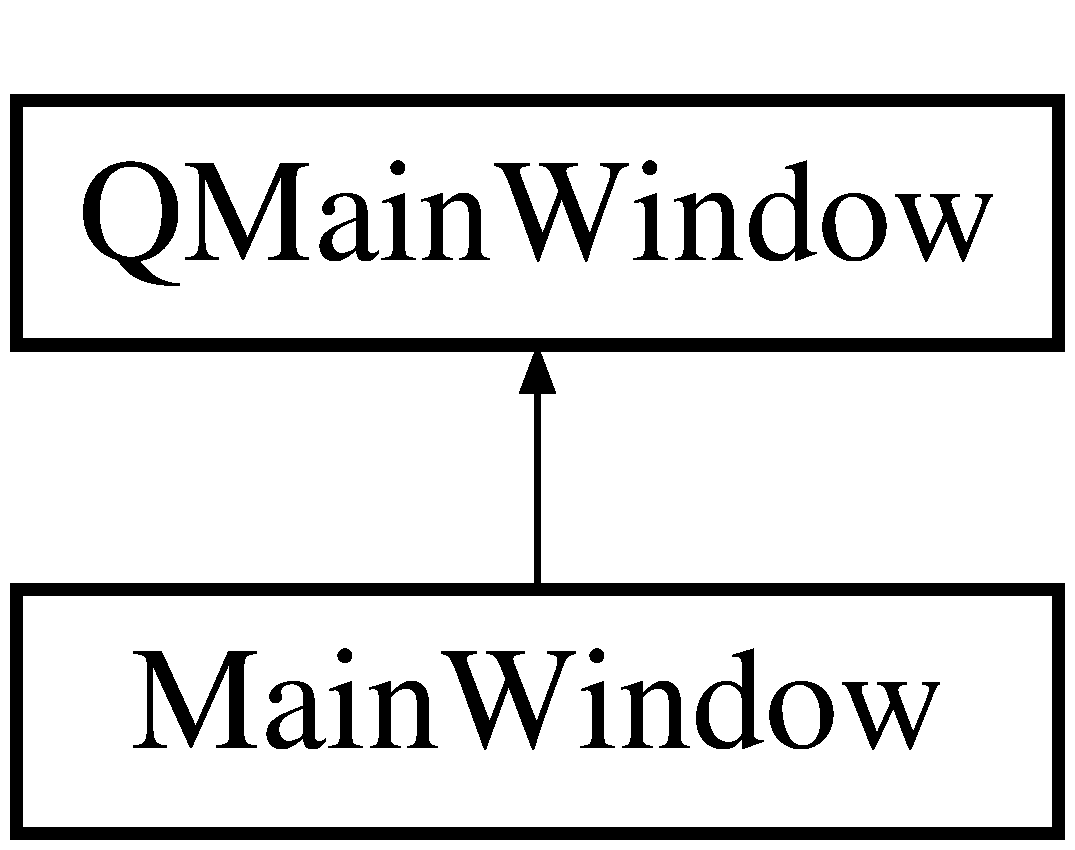
\includegraphics[height=2.000000cm]{classMainWindow}
\end{center}
\end{figure}
\subsection*{Public Member Functions}
\begin{DoxyCompactItemize}
\item 
\mbox{\Hypertarget{classMainWindow_a8b244be8b7b7db1b08de2a2acb9409db}\label{classMainWindow_a8b244be8b7b7db1b08de2a2acb9409db}} 
{\bfseries Main\+Window} (Q\+Widget $\ast$parent=0)
\end{DoxyCompactItemize}


The documentation for this class was generated from the following files\+:\begin{DoxyCompactItemize}
\item 
\hyperlink{mainwindow_8h}{mainwindow.\+h}\item 
\hyperlink{mainwindow_8cpp}{mainwindow.\+cpp}\end{DoxyCompactItemize}

\hypertarget{structnode}{}\section{node Struct Reference}
\label{structnode}\index{node@{node}}


structure representing the node of the tree  


\subsection*{Public Attributes}
\begin{DoxyCompactItemize}
\item 
\mbox{\Hypertarget{structnode_a2d890bb9f6af0ffd73fe79b21124c2a2}\label{structnode_a2d890bb9f6af0ffd73fe79b21124c2a2}} 
int \hyperlink{structnode_a2d890bb9f6af0ffd73fe79b21124c2a2}{data}
\begin{DoxyCompactList}\small\item\em real data element for the node \end{DoxyCompactList}\item 
\mbox{\Hypertarget{structnode_ad3d475f22776899938bbca39b65f2414}\label{structnode_ad3d475f22776899938bbca39b65f2414}} 
bool \hyperlink{structnode_ad3d475f22776899938bbca39b65f2414}{color}
\begin{DoxyCompactList}\small\item\em bool representing the color of node on red Black tree \end{DoxyCompactList}\item 
\mbox{\Hypertarget{structnode_a7cbff55ff448f557223f79299056e9b1}\label{structnode_a7cbff55ff448f557223f79299056e9b1}} 
\hyperlink{structnode}{node} $\ast$ \hyperlink{structnode_a7cbff55ff448f557223f79299056e9b1}{left}
\begin{DoxyCompactList}\small\item\em links to the left child , right child and the parent node \end{DoxyCompactList}\item 
\mbox{\Hypertarget{structnode_afafc72df7ea24f355ad3abb32a331689}\label{structnode_afafc72df7ea24f355ad3abb32a331689}} 
\hyperlink{structnode}{node} $\ast$ {\bfseries right}
\item 
\mbox{\Hypertarget{structnode_a2d2ad84813baa5e30cb01c8a44dde540}\label{structnode_a2d2ad84813baa5e30cb01c8a44dde540}} 
\hyperlink{structnode}{node} $\ast$ {\bfseries parent}
\end{DoxyCompactItemize}


\subsection{Detailed Description}
structure representing the node of the tree 

The documentation for this struct was generated from the following file\+:\begin{DoxyCompactItemize}
\item 
Q1.\+cpp\end{DoxyCompactItemize}

\hypertarget{classTrie}{}\section{Trie Class Reference}
\label{classTrie}\index{Trie@{Trie}}


class for \hyperlink{classTrie}{Trie} Structure  




{\ttfamily \#include $<$trie.\+h$>$}

\subsection*{Public Member Functions}
\begin{DoxyCompactItemize}
\item 
\mbox{\Hypertarget{classTrie_a6af57e9f25d0d0a2d59eea5a4a802908}\label{classTrie_a6af57e9f25d0d0a2d59eea5a4a802908}} 
\hyperlink{classTrie_a6af57e9f25d0d0a2d59eea5a4a802908}{Trie} ()
\begin{DoxyCompactList}\small\item\em A class construction to initialize the root of trie. \end{DoxyCompactList}\item 
bool \hyperlink{classTrie_a504580e3f2302333ec5f0bbfbb7d72b9}{insert} (Q\+String word, Q\+String meaning)
\begin{DoxyCompactList}\small\item\em A public membr function to insert the node/ new data into the trie. \end{DoxyCompactList}\item 
Q\+String \hyperlink{classTrie_a109938f88ed193f5e269d99d8d1931ca}{get\+Meaning} (Q\+String str)
\begin{DoxyCompactList}\small\item\em A membr function to get value stored in trie. \end{DoxyCompactList}\item 
\mbox{\Hypertarget{classTrie_a90c8ea2ede015711805332c3b6882e59}\label{classTrie_a90c8ea2ede015711805332c3b6882e59}} 
void \hyperlink{classTrie_a90c8ea2ede015711805332c3b6882e59}{load\+Data\+In\+Trie} ()
\begin{DoxyCompactList}\small\item\em A membr function to store the data from file into the trie. \end{DoxyCompactList}\end{DoxyCompactItemize}


\subsection{Detailed Description}
class for \hyperlink{classTrie}{Trie} Structure 

A more elaborate class description. 

\subsection{Member Function Documentation}
\mbox{\Hypertarget{classTrie_a109938f88ed193f5e269d99d8d1931ca}\label{classTrie_a109938f88ed193f5e269d99d8d1931ca}} 
\index{Trie@{Trie}!get\+Meaning@{get\+Meaning}}
\index{get\+Meaning@{get\+Meaning}!Trie@{Trie}}
\subsubsection{\texorpdfstring{get\+Meaning()}{getMeaning()}}
{\footnotesize\ttfamily Q\+String Trie\+::get\+Meaning (\begin{DoxyParamCaption}\item[{Q\+String}]{str }\end{DoxyParamCaption})\hspace{0.3cm}{\ttfamily [inline]}}



A membr function to get value stored in trie. 


\begin{DoxyParams}{Parameters}
{\em str} & string whose meaning to find \\
\hline
\end{DoxyParams}
\begin{DoxyReturn}{Returns}
Q\+String G\+UI supported String 
\end{DoxyReturn}
\mbox{\Hypertarget{classTrie_a504580e3f2302333ec5f0bbfbb7d72b9}\label{classTrie_a504580e3f2302333ec5f0bbfbb7d72b9}} 
\index{Trie@{Trie}!insert@{insert}}
\index{insert@{insert}!Trie@{Trie}}
\subsubsection{\texorpdfstring{insert()}{insert()}}
{\footnotesize\ttfamily bool Trie\+::insert (\begin{DoxyParamCaption}\item[{Q\+String}]{word,  }\item[{Q\+String}]{meaning }\end{DoxyParamCaption})\hspace{0.3cm}{\ttfamily [inline]}}



A public membr function to insert the node/ new data into the trie. 


\begin{DoxyParams}{Parameters}
{\em word} & word whose meaning is to be stored \\
\hline
{\em meaning} & meaning of the given word \\
\hline
\end{DoxyParams}
\begin{DoxyReturn}{Returns}
bool whether inserted successfully or not 
\end{DoxyReturn}


The documentation for this class was generated from the following files\+:\begin{DoxyCompactItemize}
\item 
\hyperlink{trie_8h}{trie.\+h}\item 
\hyperlink{trie_8cpp}{trie.\+cpp}\end{DoxyCompactItemize}

\chapter{File Documentation}
\hypertarget{main_8cpp}{}\section{main.\+cpp File Reference}
\label{main_8cpp}\index{main.\+cpp@{main.\+cpp}}


this file will contain all required definitions and basic utilities functions.  


{\ttfamily \#include \char`\"{}mainwindow.\+h\char`\"{}}\newline
{\ttfamily \#include $<$Q\+Application$>$}\newline
\subsection*{Functions}
\begin{DoxyCompactItemize}
\item 
\mbox{\Hypertarget{main_8cpp_a0ddf1224851353fc92bfbff6f499fa97}\label{main_8cpp_a0ddf1224851353fc92bfbff6f499fa97}} 
int {\bfseries main} (int argc, char $\ast$argv\mbox{[}$\,$\mbox{]})
\end{DoxyCompactItemize}


\subsection{Detailed Description}
this file will contain all required definitions and basic utilities functions. 

\begin{DoxyAuthor}{Author}
Karanpreet Singh
\end{DoxyAuthor}
\begin{DoxyDate}{Date}
04/08/19 
\end{DoxyDate}

\hypertarget{mainwindow_8cpp}{}\section{mainwindow.\+cpp File Reference}
\label{mainwindow_8cpp}\index{mainwindow.\+cpp@{mainwindow.\+cpp}}


this file will contain all required definitions and basic utilities functions.  


{\ttfamily \#include \char`\"{}mainwindow.\+h\char`\"{}}\newline
{\ttfamily \#include \char`\"{}ui\+\_\+mainwindow.\+h\char`\"{}}\newline
{\ttfamily \#include $<$Q\+Message\+Box$>$}\newline


\subsection{Detailed Description}
this file will contain all required definitions and basic utilities functions. 

\begin{DoxyAuthor}{Author}
Karanpreet Singh
\end{DoxyAuthor}
\begin{DoxyDate}{Date}
04/08/19 
\end{DoxyDate}

\hypertarget{mainwindow_8h}{}\section{mainwindow.\+h File Reference}
\label{mainwindow_8h}\index{mainwindow.\+h@{mainwindow.\+h}}


this file will contain all required definitions and basic utilities functions.  


{\ttfamily \#include $<$Q\+Main\+Window$>$}\newline
{\ttfamily \#include \char`\"{}trie.\+h\char`\"{}}\newline
\subsection*{Classes}
\begin{DoxyCompactItemize}
\item 
class \hyperlink{classMainWindow}{Main\+Window}
\end{DoxyCompactItemize}


\subsection{Detailed Description}
this file will contain all required definitions and basic utilities functions. 

\begin{DoxyAuthor}{Author}
Karanpreet Singh
\end{DoxyAuthor}
\begin{DoxyDate}{Date}
04/08/19 
\end{DoxyDate}

\hypertarget{trie_8cpp}{}\section{trie.\+cpp File Reference}
\label{trie_8cpp}\index{trie.\+cpp@{trie.\+cpp}}


this file will contain all required definitions and basic utilities functions.  


{\ttfamily \#include $<$bits/stdc++.\+h$>$}\newline
{\ttfamily \#include \char`\"{}Q\+String\char`\"{}}\newline
{\ttfamily \#include \char`\"{}trie.\+h\char`\"{}}\newline
{\ttfamily \#include \char`\"{}Q\+Debug\char`\"{}}\newline
\subsection*{Functions}
\begin{DoxyCompactItemize}
\item 
\hyperlink{structnode}{node} $\ast$ \hyperlink{trie_8cpp_a2d0f25676b21fcd44a1d80fab3975e06}{initialize} ()
\end{DoxyCompactItemize}


\subsection{Detailed Description}
this file will contain all required definitions and basic utilities functions. 

\begin{DoxyAuthor}{Author}
Karanpreet Singh
\end{DoxyAuthor}
\begin{DoxyDate}{Date}
04/08/19 
\end{DoxyDate}


\subsection{Function Documentation}
\mbox{\Hypertarget{trie_8cpp_a2d0f25676b21fcd44a1d80fab3975e06}\label{trie_8cpp_a2d0f25676b21fcd44a1d80fab3975e06}} 
\index{trie.\+cpp@{trie.\+cpp}!initialize@{initialize}}
\index{initialize@{initialize}!trie.\+cpp@{trie.\+cpp}}
\subsubsection{\texorpdfstring{initialize()}{initialize()}}
{\footnotesize\ttfamily \hyperlink{structnode}{node}$\ast$ initialize (\begin{DoxyParamCaption}{ }\end{DoxyParamCaption})}

This method will be used initialize the node s \begin{DoxyAuthor}{Author}
Karanpreet Singh 
\end{DoxyAuthor}
\begin{DoxyDate}{Date}
02/09/19 
\end{DoxyDate}

\hypertarget{trie_8h}{}\section{trie.\+h File Reference}
\label{trie_8h}\index{trie.\+h@{trie.\+h}}


this file will contain all required definitions and basic utilities functions.  


\subsection*{Classes}
\begin{DoxyCompactItemize}
\item 
struct \hyperlink{structnode}{node}
\begin{DoxyCompactList}\small\item\em structure representing the node of the tree \end{DoxyCompactList}\item 
class \hyperlink{classTrie}{Trie}
\begin{DoxyCompactList}\small\item\em class for \hyperlink{classTrie}{Trie} Structure \end{DoxyCompactList}\end{DoxyCompactItemize}
\subsection*{Functions}
\begin{DoxyCompactItemize}
\item 
\hyperlink{structnode}{node} $\ast$ \hyperlink{trie_8h_a2d0f25676b21fcd44a1d80fab3975e06}{initialize} ()
\end{DoxyCompactItemize}


\subsection{Detailed Description}
this file will contain all required definitions and basic utilities functions. 

\begin{DoxyAuthor}{Author}
Karanpreet Singh
\end{DoxyAuthor}
\begin{DoxyDate}{Date}
04/08/19 
\end{DoxyDate}


\subsection{Function Documentation}
\mbox{\Hypertarget{trie_8h_a2d0f25676b21fcd44a1d80fab3975e06}\label{trie_8h_a2d0f25676b21fcd44a1d80fab3975e06}} 
\index{trie.\+h@{trie.\+h}!initialize@{initialize}}
\index{initialize@{initialize}!trie.\+h@{trie.\+h}}
\subsubsection{\texorpdfstring{initialize()}{initialize()}}
{\footnotesize\ttfamily \hyperlink{structnode}{node}$\ast$ initialize (\begin{DoxyParamCaption}{ }\end{DoxyParamCaption})}

This method will be used initialize the node s \begin{DoxyAuthor}{Author}
Karanpreet Singh 
\end{DoxyAuthor}
\begin{DoxyDate}{Date}
02/09/19 
\end{DoxyDate}

%--- End generated contents ---

% Index
\backmatter
\newpage
\phantomsection
\clearemptydoublepage
\addcontentsline{toc}{chapter}{Index}
\printindex

\end{document}
